\documentclass[]{article}
\usepackage[UTF8]{ctex}
\usepackage[a4paper,left=10mm,right=10mm,bottom=10mm,top=10mm]{geometry}
\usepackage{graphicx}
\usepackage{float}
\usepackage{amsmath,amsfonts,amssymb,amsthm}
\usepackage{array,color}
% \usepackage{times}
% \usepackage{latexsym}
%opening
\title{OSlab1-Report}
\author{陈昱衡 521021910939}
\date{\today}

\begin{document}

\maketitle



\section{Copy}
\begin{enumerate}
    \item [1] \textbf{Basic requirement:} Write a C program that forks two processes to copy file, one for reading
    from a source file, and the other for writing into a destination file, using system calls. These two
    processes communicate using \textbf{pipe} system call. The name of source file and destination file are
    to be specified as command line arguments.
    \item [2] \textbf{Advanced requirement:}
        \begin{itemize}
            \item Use a suitable size of buffer in order to copy faster.
            \item Use various system calls for time to compare the performance of this program with at least
            8 different buffer size.
            \item Use graphic tools or programs for plotting the execution time over different buffer size and
            try to explain the result.            
        \end{itemize}
    \item [3] \textbf{More details of requirement:}
        \begin{itemize}
            \item Source file name: Copy.c
            \item Executable file name: Copy
            \item Command line: ./Copy <InputFile> <OutputFile> <BufferSize>
        \end{itemize}
\end{enumerate}
\subsection*{Harvest and Reflections}
\begin{enumerate}
    \item While dealing with this problem, I get more familiar with the lib functions and linux syscalls.
    \item I am also be equipped with more skills such as writing a makefile, counting the time consumed by the programme and some other tricks such as graphing tools.

\end{enumerate}

\subsection*{Solution}
\begin{enumerate}
    \item The first task is to cerate two child process. Create like this:\par
    % \framebox[10em][r]{Test box}\\[1ex] 
    % \setlength{\fboxrule}{1.6pt} 
    % \setlength{\fboxsep}{1em} 
    % \framebox[40em][c]{
    % \begin{verbatim} 
    %     pid\_t pid1 = fork();
    %     pid\_t pid2 = fork();
    %     if(getpid() == pid1) ...
    %     if(getpid() == pid2) ...
    % \end{verbatim}
    % }

    
    \begin{verbatim} 
        pid\_t pid1 = fork();
        pid\_t pid2 = fork();
        if(getpid() == pid1) ...
        if(getpid() == pid2) ...
    \end{verbatim}
    is wrong.We can use a loop or just call fork() separately.
    \item Then I met some problem.When I tried to use \textbf{diff} command to compare the files.I get the input below:
    \begin{verbatim}
        $ diff sample_data1.out sample/sample_data.in
        129,132c129
        < 28 4 9 23 22 5 24 25 11 3 2 10 14 11 4 28 1 17 4 27 25 25 5 8 21 7 6 2 16 27 18 6 2 19 
        29 16 17 15 12 28 18 14 8 24 25 4 14 19 22 18 8 9 13 14 17 27 13 24 29 21 13 9 27 7 29 
        26 24 8 3 6 6 13 12 6 7 0 11 22 19 25 10 19 4 16 3 14 13 8 0 4 29 13 14 26 21 13 14 7 13 
        17 5 19 22 17 25 0 17 28 22 28 15 24 18 12 2 13 26 7 22 26 12 21 1 26 10 22 1 24 25 6 16 
        21 28 28 25 16 0 2 1 21 3 1 24 11 4 4 28 3 9 8 8 14 29 4 27 26 18 21 11 13 19 27 27 17 17 
        22 26 17 24 27 1 20 20 25 1 24 21 29 19 1 7 19 7 29 24 4 17 12 18 28 18 7 18 15 17 5 29 5 
        15 23 2 8 5 22 3 6 8 17 28 28 10 27 17 17 26 3 14 13 16 2 4 26 1 22 11 10 19 10 15 26 25 9 
        4 23 1 0 21 2 17 19 22 19 17 
        < 1 6 5 5 12 19 13 6 15 9 8 7 12 10 26 14 26 15 1 5 19 24 29 11 16 23 20 5 15 9 14 16 8 20 
        13 20 1 26 27 16 27 27 15 9 29 3 23 25 18 25 23 0 11 14 11 27 7 2 25 14 11 9 22 19 21 6 2 
        22 24 29 0 22 18 15 23 17 19 9 5 7 4 20 7 15 4 11 5 3 13 0 9 16 1 1 6 23 29 0 15 24 29 8 8 
        9 23 1 26 12 2 23 12 6 13 11 14 9 22 11 12 27 11 21 14 12 15 12 27 14 
        < 12 5 0 3 13 8 12 6 2 0 11 4 24 15 3 7 18 9 17 11 20 21 0 23 13 14 27 28 26 25 4 8 0 5 11 
        5 5 15 3 29 16 14 26 10 21 29 17 10 0 26 13 20 18 13 13 23 28 10 13 16 27 17 17 27 14 20 2 
        20 6 6 11 22 12 7 24 4 28 11 6 28 0 19 10 18 24 15 3 22 26 16 1 15 25 18 13 10 8 7 22 14 5 
        3 28 18 11 22 14 9 26 12 0 26 1 10 6 25 18 9 10 6 17 3 21 12 21 4 22 21 
        < 4 14 28 9 18 26 19 21 19 25 22 7 7 14 3 0 17 1 18 5 2 20 11 19 23 2 1 14 29 24 27 3 0 25 
        4 10 22 16 1 3 11 16 10 19 0 5 11 17 6 29 22 8 19 3 27 12 28 20 18 27 14 16 22 7 11 26 17 
        25 12 11 28 16 27 0 5 27 5 16 7 3 8
        \ 文件尾没有换行符
        ---
        > 28 4 9 23 22 5 24 25 11 3 2 10 14 11 4 28 1 17 4 27 25 25 5 8 21 7 6 2 16 27 18 6 2 19 
        29 16 17 15 12 28 18 14 8 24 25 4 14 19 22 18 8 9 13 14 17 27 13 24 29 21 13 9 27 7 29 26
        24 8 3 6 6 13 12 6 7 0 11 22 19 25 10 19 4 16 3 14 13 8 0 4 29 13 14 26 21 13 14 7 13 17 
        5 19 22 17 25 0 17 28 22 28 15 24 18 12 2 13 26 7 22 26 12 21 1 26 10 22 1 24 
        \ 文件尾没有换行符
    \end{verbatim}
    \par 
    I tried to figure out the reason and I think that the uncleared buf gave rise to the problem.And initially I declared a char* and call malloc to apply for heap.
    But finally I just tried the char[] and it works well.\par 
    I wonder if it is because the c                                                                                                                                                                                                                                                                                                                                                                                                                                                                                                                                                                                                                                                                                                                                                                                                                                                                                                                                                                                                                                                                                                                                                                                                                                                                                                                                                                                                                                                                                                                                                                                                                                                                                                                                                                                                                                                                                                                                                                                                                                                                                                                                                                                                                                                                                                                                                                                                                                                                                                                                                                                                                                                                                                                                                                                                                                                                                                                                                                                                                                                                                                                                                                                                                                                                                                                                                                                                                                                                                                                                                                                                                                                    hild process and the parent process shared the same heap?\par 
\end{enumerate}

\subsection*{Performance Analysis}
The time consumed with different buffer size:
\begin{figure}[H]
    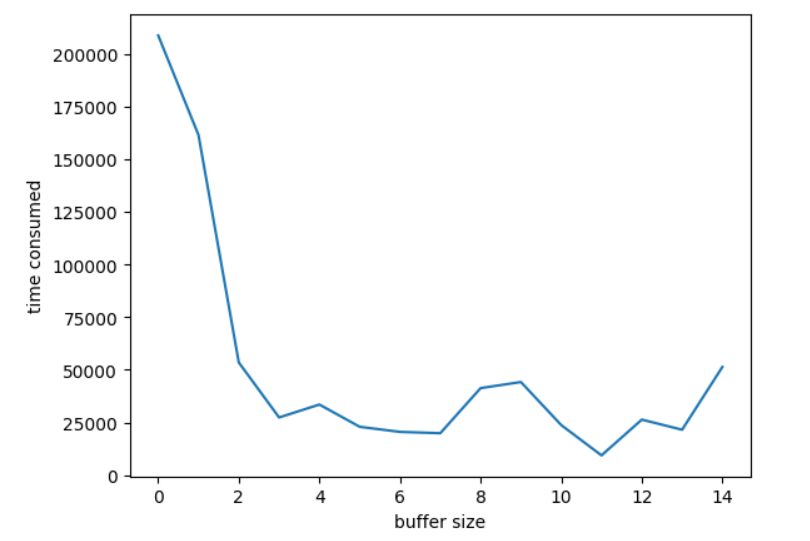
\includegraphics[scale = 0.5]{2023-03-24-19-20-55.png}
\end{figure}
We can see that as the buffer size grow , the time consumed decreases and the increase.I surf the internet and get the idea that the usual Unix and Linux buffer size is 4kb.So, if the buffersize is too small , we have to write many times which cost a lot of time.And, if the buffersize is too big, the time of writing one time is longer . So the time cost first decrease and then increase.
\par 

\section{Shell}
\begin{enumerate}
    \item [1] \textbf{Basic requirement:} Write a shell-like program that illustrates how Linux spawns processes. It
    should handle the commands with arguments and the commands connected by pipes. \textbf{Example} :
    ls -l | wc. Use dup system call to redirect I/O.
    
    \item [2] \textbf{Advanced requirement:}  Write the above shell program as a server. When the server is
    running, clients are allowed to connect to the server and run the commands. The communication
    between client and server should be implemented using Internet-domain socket.
    
    \item[3] \textbf{More details of requirement:} 
    \begin{itemize}
        \item Server should work in an infinite loop.
        \item Using messages between server and client is suggested.
        \item There must be a command exit to disconnect the connection between server and client.
        \item There may be more than one ‘|’ in the command line.
        \item Try to support more than one client.
        \item Server will be tested by using telnet, the command line is as follows.
        \item Command line for telnet: telnet <IPAddress> <Port>
        \item Source file name: shell.c
        \item Executable file name: shell
        \item Command line: ./shell <Port>
    \end{itemize}
\end{enumerate}

\subsection*{Harvest and Reflections}
    \begin{enumerate}
        \item [1] During the process of solving this problem,I get aware of the importance of "Unit test".This task Shell can be seen as 
        a combination of different utilities,such as local shell,socket programming,pipe programming.So I just realize this functions separately and finally put them together.
        I think this conforms to Unix philosophy.
        \item[2] During the loop of coding ,running, testing,debugging and then coding again,I get a further understanding of how to use pipe,dup,fork syscalls.Since programming under kernel is kind of difficult,
        ,I think that maybe I have tried some useful ways of tracking errors.
        \item[3] Also,aside from enhancing my programming abilities, I know more about Linux command,such as POSIX.I understand how the shell works in a more profound way.
    \end{enumerate}

\subsection*{Solution}
        \begin{enumerate}
            \item [\textbf{Step 1}] \textbf{local shell without redirection}
            \begin{itemize}
                \item First, I define several micros to represent the length limitation of command line input under Linux.
                \item Then,I realize the function \textbf{parseLine()} to get each separate parameters.This function gets use of the library function \textbf{strtok\_r()},
                since strtok() is not safe.I read all the parameters at one time and record them in an array.Besides,in parseLine(), there are several lines of error judgement and management.Such as "Missing cmd before pipe","Missing cmd after pipe".
                \item Then,in the main function,there is a while(1) infinite loop,keeping reading input from stdin and process them.
                \item After getting all the parameters,I call \textbf{fork()} to create a child process in which I redirect IO and call \textbf{execvp()} to run command.It is such a abrupt thought to redirect IO in parent process.I initially took this realization,definitely I was fooled by no output from shell as if my computer was undergoing a dead lock.
                There is also a error check in child process,since the execvp() will never return to the caller,so we can add error detection code just under the execvp() call.
                \item In the parent process, we can just \textbf{wait(NULL)} in this step.
            \end{itemize}
            
            \item[\textbf{Step 2}] \textbf{Cd command}
            \begin{itemize}
                \item This step, I was really met with some difficulty."cd" command went wrong!But how could this have been?
                First I thought that "cd" is short for "\textbf{chdir}",so I use chdir instead.But things did not change for the better.
                So I STFW.I got the answer,"cd" is realized specially in the shell program.
                \item I use the \textbf{getcwd()} syscall and the \textbf{chdir()} syscall to get the current working
                directory and to change to another directory.During this period,I first put the \textbf{chidr()} call
                in the child process wrongly so the directory wasn't changed in main loop.I correct this fault and then the 
                program workded the way I designed.\par 
            \end{itemize}

            \item[\textbf{Step 3}]  \textbf{local shell with redirection}
            \begin{itemize}
                \item This step, I intend to realize pipe and redirection by making use of \textbf{pipe()} , \textbf{dup2()} and \textbf{close()} syscall.
                \item I declare an int variable cnt to mark the number of command nad a double-dimension array fd[cnt][]. The ith command redirect it stdin to fd[i-1][0],and redirect it stdout to fd[i][1] while the first command keeps its stdin without redirecting.
                \item In this step, we need cnt child processes,each executes a command.But how to create these processes? Can we just keep coding "pid\_t pid1 = fork(), pid2 = fork() $\cdots$ " in a row? No! I was trapped here owing to my thoughtlessness.So I get really incomprehensible output.
                The correct way to create cnt child processing is to use "for loop".
                \item The most challenging part of this step is redirect IO.But thankfully,the instructor had offered some hints.
                \item There are some details wa have to pay attention to,mostly error detection,such as pipe() failure or fork() failure.
                
            \end{itemize}

            \item[\textbf{Step 4}] \textbf{A server which can be accessed by different clients}
            \begin{itemize}
                \item This step,I realize the utility with calls to \textbf{socket()},\textbf{accept()},\textbf{connect()},\textbf{recv()},\textbf{send()} and some other syscalls.
                \item First, I include some special head files.
                \item Then, I create several child processes to communicate with certain client.
                \item In each child process, I use an infinite loop in which there are \textbf{recv()} and \textbf{send()} syscalls to chat with client.The loop will be broken by certain input ,for instance "exit".
                \item Last,in the parent process ,just \textbf{close(connect\_socket\_fd)} ,\textbf{\emph{do not wait(NULL)}}!
            \end{itemize}

            \item[\textbf{Step 5}] \textbf{Combination}
            \begin{itemize}
                \item Well, I have realize all the unit functions I am about to use.So this step,what I need to do is combination.
                \item There are some details,replacing the \textbf{read()} syscall in step1 with \textbf{recv()} as we need to get input from client.
                \item In child process, timely \textbf{exit(0)} or \textbf{exit(1)} is important. 
            \end{itemize}
            
        \end{enumerate}
\subsection*{Show}
For showing how my shell works, I have tried to use jupyter, but I failed.So I just gave tmux a try,and it works as below:
\begin{figure}[H]
    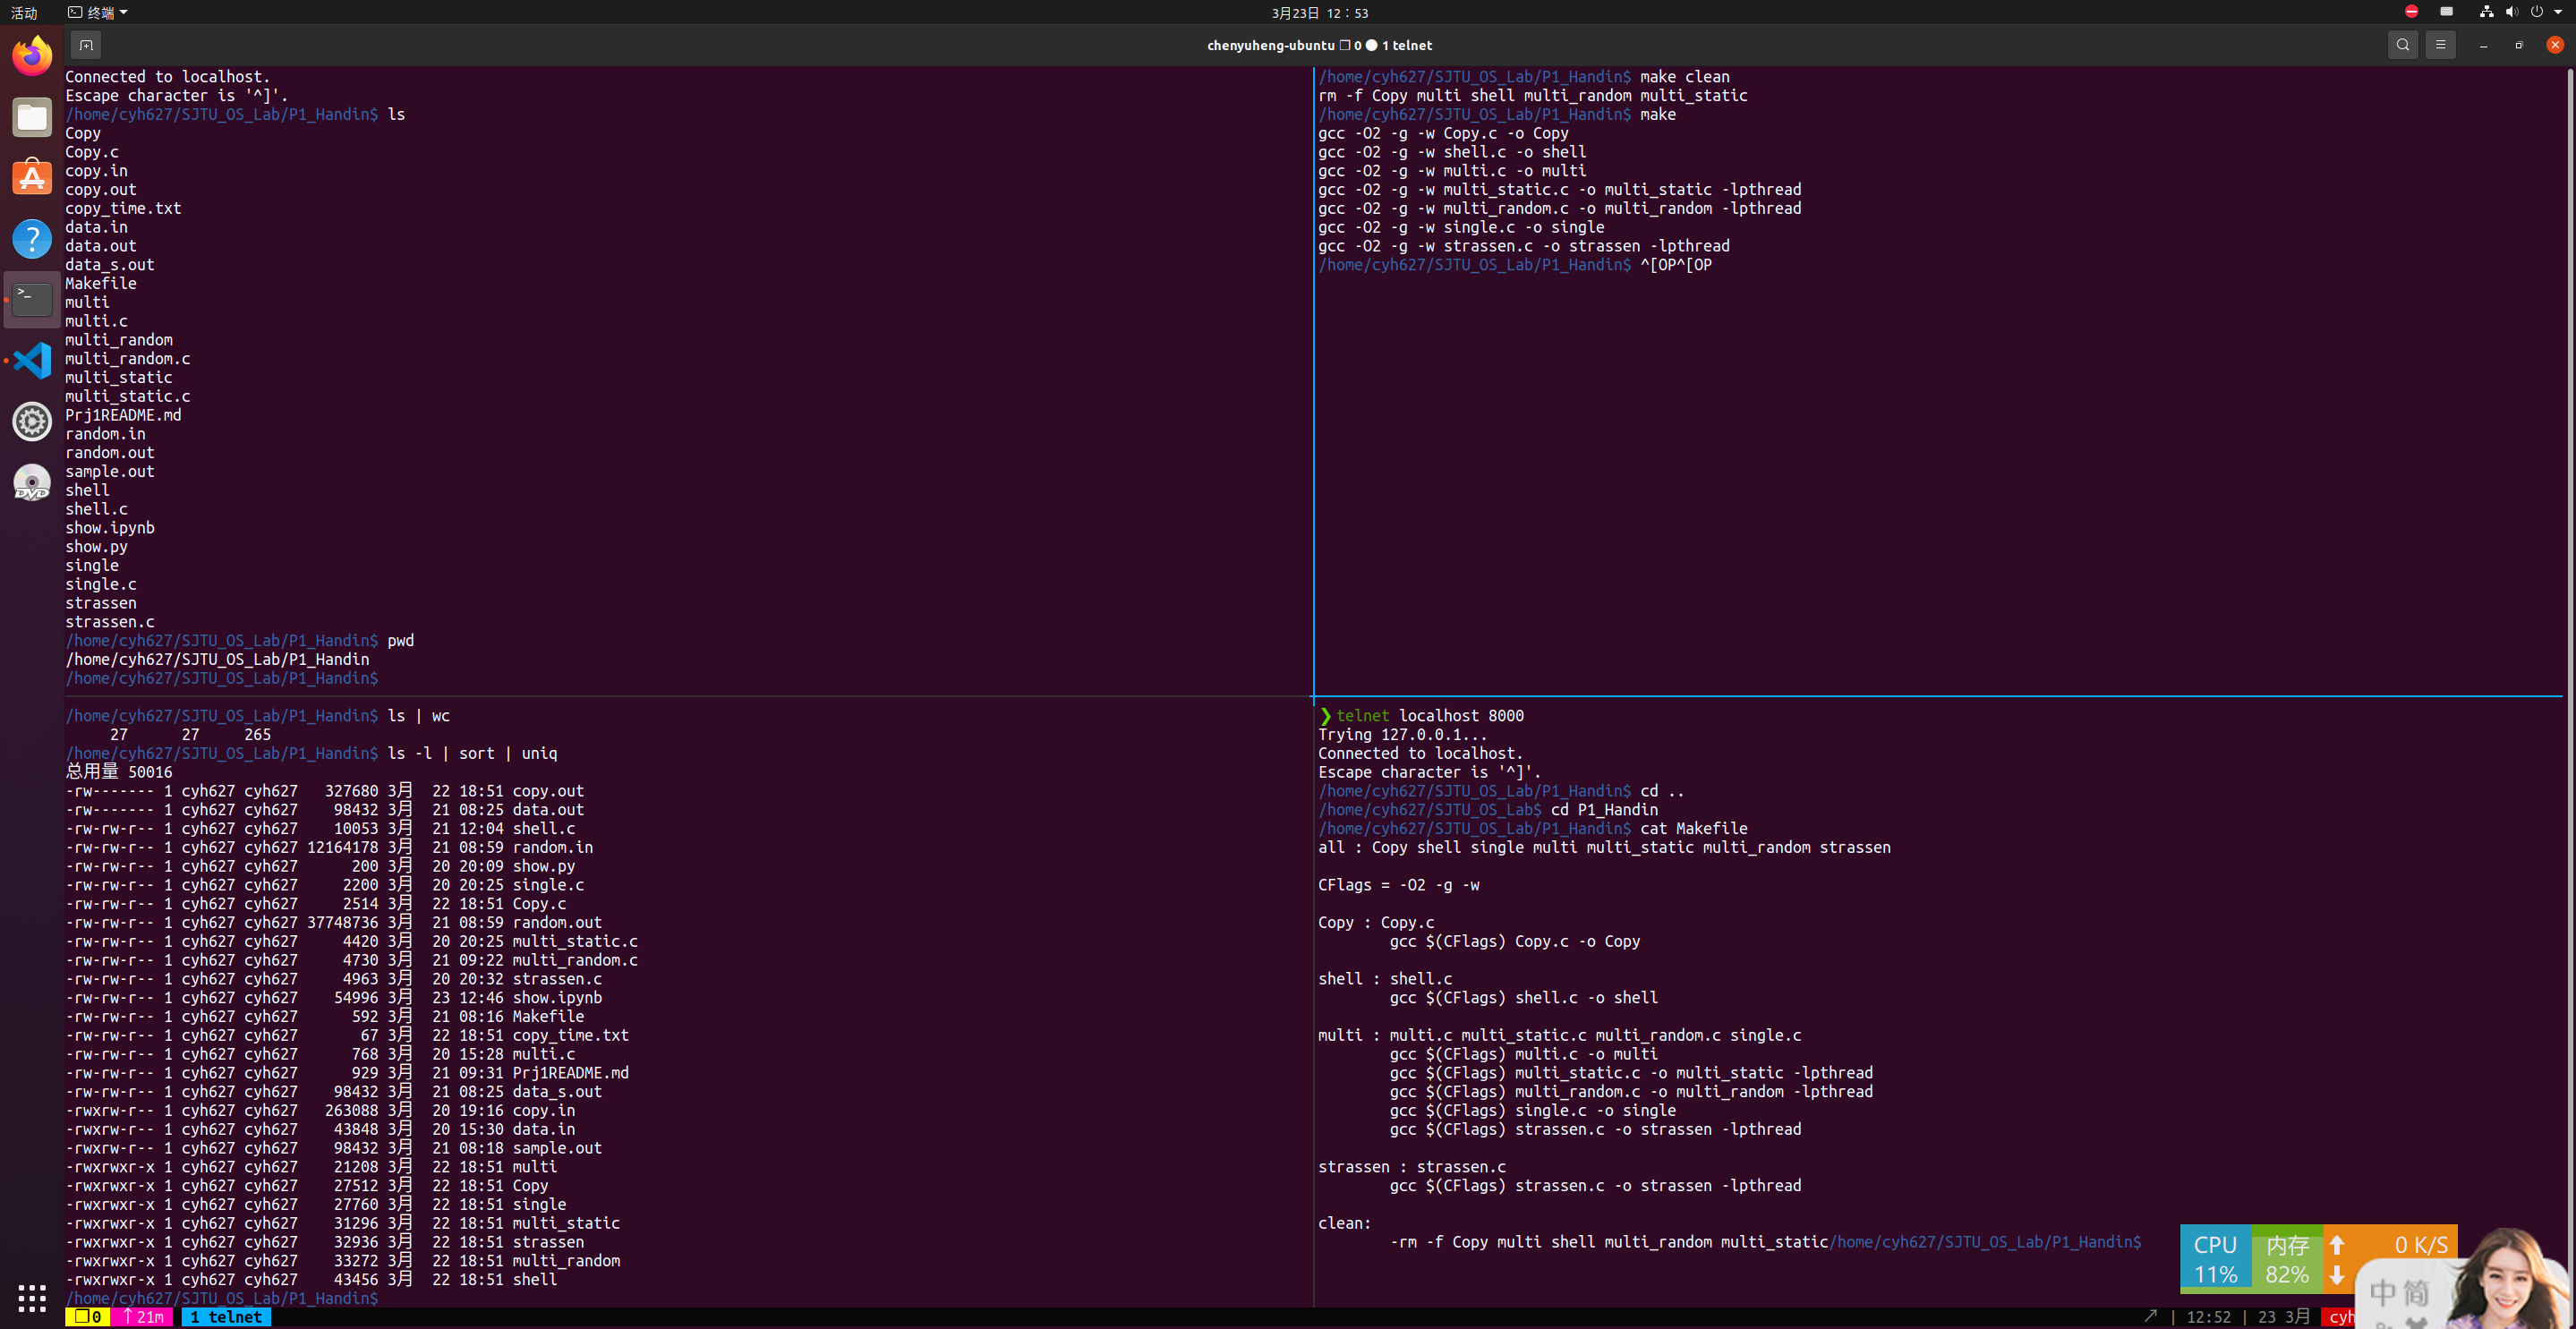
\includegraphics[scale = 0.25]{2023-03-23-12-52-48.png}
\end{figure}

\section{Matrix Multiplication}
\begin{enumerate}
    \item \textbf{Basic requirement:} Matrix multiplication is widely used in scientific computing. From linear
    algebra, it’s known that partition matrix can be used to do matrix multiplication. The main idea
    of this task is to implement matrix multiplication using any matrix partition based algorithm
    you like with time complexity O($n^3$). Please follow the requirement below.
    \begin{itemize}
        \item Find a partition-based matrix multiplication algorithm with time complexity of O($n^3$)
        \item Implement a single-thread program for matrix multiplication
        \item Implement a multi-thread program for matrix multiplication with the help of partition
        matrix.
    \end{itemize}
    \item \textbf{Advanced requirement:}Compare the performance of implementations with different number
    of threads and different size of matrix. Draw a diagram and try to explain the result. Please use
    at least 6 different numbers of threads and 8 different sizes of matrix.
    
\end{enumerate}
\subsection*{Harvests and Reflections}
\begin{enumerate}
    \item[1] I recover how the partitioning of matrix works in accelerating the matrix multiplication.
    \item[2] I also get to know the most efficient algorithm "Strassen algorithm" of matrix multiplication with time complexity of O($n^{\log_2 7}$) 
    \item[3] I get familiar with multi-thread programming under linux.
    \item[4] I get to know some frustrating thing about multi-thread programming and the way to prevent it.
    \item[5] There is a funny thing I want to mention:I create up to 32768 threads to calculate the matrix.Then I get fully aware of the strengths of multi-threads.To make full use of the multi-cpus, the thread number is supposed to be less than the cpu number.
\end{enumerate}

\subsection*{Solution}
\begin{enumerate}
    \item[\textbf{Step1}] \textbf{Using multithread to do Matrix multiplication}
    \begin{itemize}
        \item I use the \textbf{ptherad.h} lib,and use the \textbf{-lpthread} gcc option to compile the source code.
        \item I declared an array of \textbf{pthread\_t} and \textbf{pthread\_attr\_t} and use \textbf{pthread\_create()} along with \textbf{pthread\_join()} to create and run different threads.
        \item To generate random numbers composing the matrix,initially I was not satisfied with the random number generators
        offered by \textbf{stdlib.h},so I tried to replace it with the asm command RDRAND offered by intel which make use of
        thermal noise inside of CPU.Here is the code:
        \begin{verbatim}
        	uint64_t random_uint64(void) {
        		uint64_t result;
        		unsigned char ok;
        		__asm__ __volatile__("rdrand %0; setc %1"
        		: "=r" (result), "=qm" (ok));
        		if (ok) {
        			return result;
        		} else {
        			// RDRAND failed, fall back to something else
        			fprintf(stderr, "generate random number failed\n");
        			return 0;
        		}
        	}
        \end{verbatim}
        \item But after I had finished coding I run the programme and the diff command to compare my answer with the standard output.
        I got a bunch of output which really startled me.There exist many different lines but each of them only had a single different element.
        It occurred to me that maybe this was due to the multithreading destroying atomicity of directives.\par 
        \item First I inserted some inline assembly code \textbf{asm volatile ("" ::: "memory");},also used the \textbf{volatile} to declare my variables.
        But it didn't work.
        \item So I STFW and get to know the \textbf{mutex}.I used the struct \textbf{pthread\_mutex\_t} and lib functions
        \textbf{pthread\_\\mutex\_lock(\&mutex)} and \textbf{pthread\_mutex\_unlock(\&mutex)} to keep the memory writing directives atomic.
        \item Also,later I was aware that there were some other detectives to keep the multithreading correct.The function "\_\_sync\_synchronize()"
        supported by compiler can reduce the times that error occurs but cannot prevent it.Or I tried to insert "\textbf{asm volatile (mfence)}",but it failed too.\par         
        \item During the process of coding,I was confronted with the error "\textbf{create thread: Cannot allocate memory}" as well.
        I combat with the error for really long time.I finally separate them and use \textbf{execvp} to call \textbf{multi\_static} which read matrix from \textbf{data.in},\textbf{multi\_random} which generate random matrix.\par 
    \end{itemize}
    \item [\textbf{Step2}] \textbf{Strassen algorithm}
    \begin{itemize}
        \item Strassen algorithm is a divide-and-conquer algorithm for matrix multiplication.It might be the most efficient algorithm for matrix multiplication with time complexity of O($n^{\log_2 7}$).
        So I tried to implement it.
        \item The process of generate all the matrixes that Strassen algorithm employs is awful and error prone. I made some mistakes at first and my upper left corner matrix appears to be all zero.
        \item The calculation process is the same as the basic algorithm,but it just need 7 threads.
        \item Last, combine all the matrixes together to get the final answer. 
    \end{itemize}
\end{enumerate}

\subsection*{Performance Analysis}
I do the matrix multiplication with 1 to 8 threads and 32 to 4096 matrix size, and get this figure:
\begin{figure}[H]
    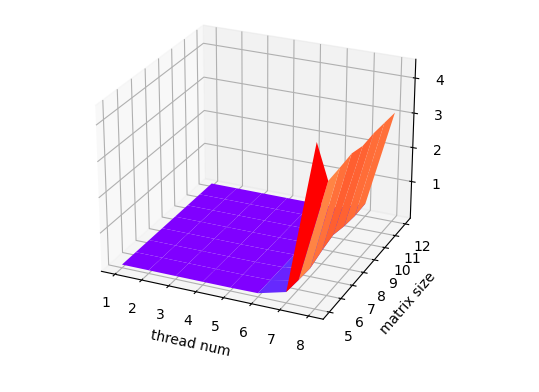
\includegraphics[scale = 0.6]{2023-03-25-13-46-38.png}
    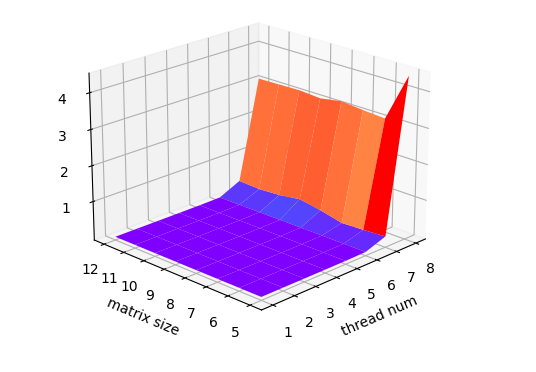
\includegraphics[scale = 0.6]{2023-03-25-13-47-06.png}
\end{figure}
Since the time cost grow exponentially as the matrix size grow, so the figure fail to show the efficiency obviously to some extent.\par 
So I draw the charts separately:
\begin{figure}[H]
    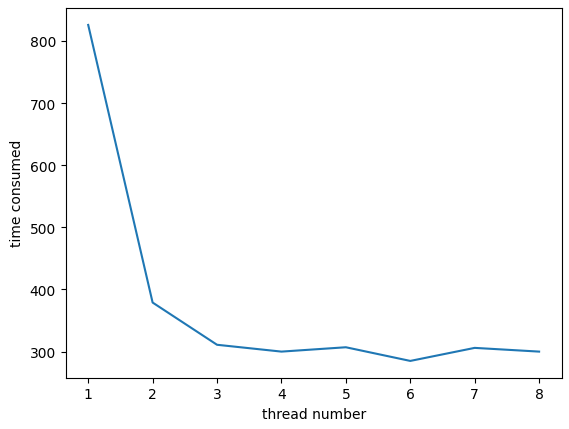
\includegraphics[scale = 0.6]{2023-03-25-13-56-26.png}
    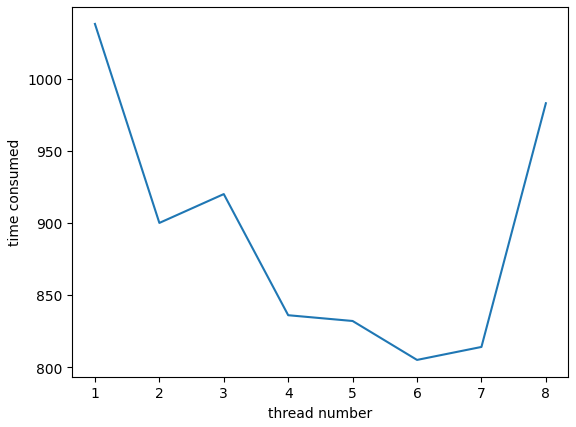
\includegraphics[scale = 0.6]{2023-03-25-13-57-34.png}
    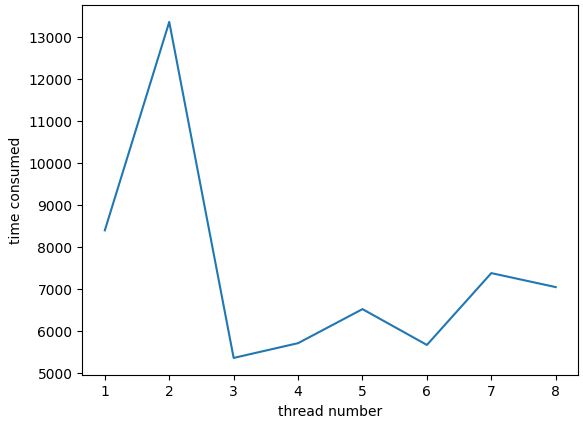
\includegraphics[scale = 0.6]{2023-03-25-13-57-52.png}
    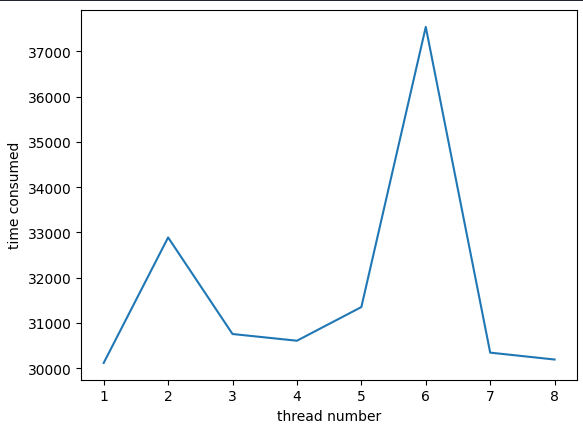
\includegraphics[scale = 0.6]{2023-03-25-13-58-09.png}
    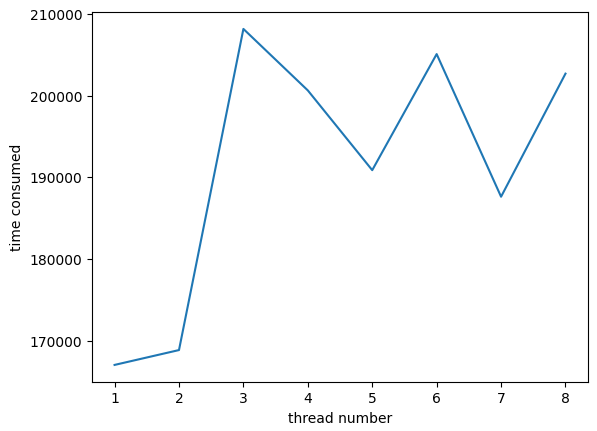
\includegraphics[scale = 0.6]{2023-03-25-13-58-20.png}
    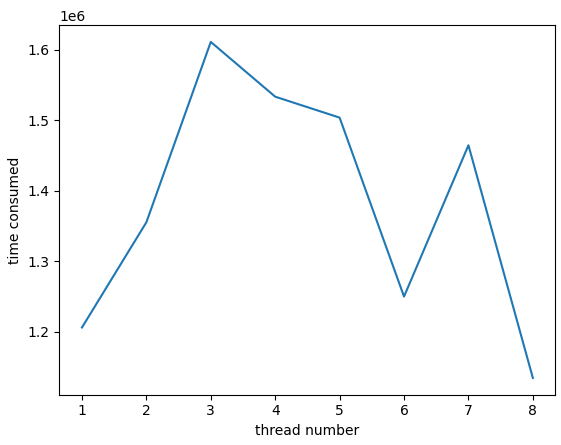
\includegraphics[scale = 0.6]{2023-03-25-13-58-35.png}
    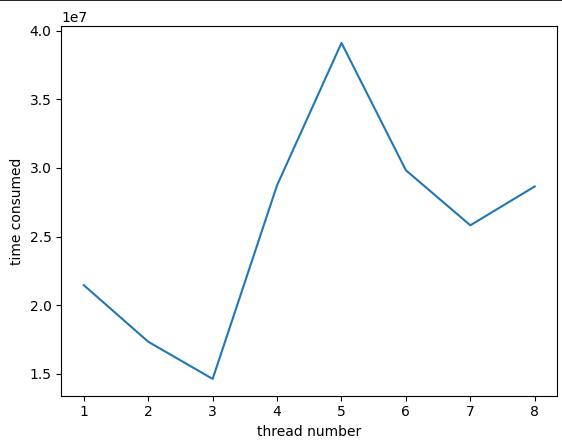
\includegraphics[scale = 0.6]{2023-03-25-13-58-44.png}
    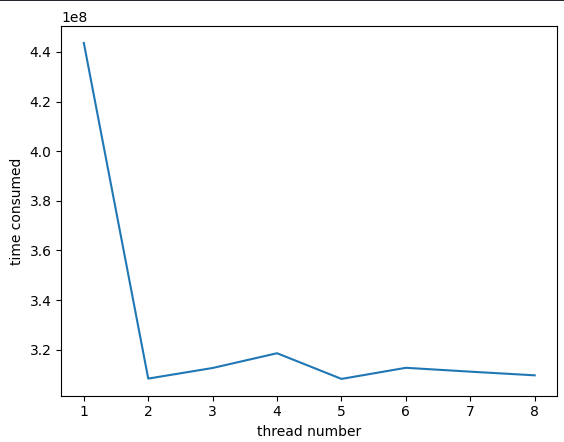
\includegraphics[scale = 0.6]{2023-03-25-13-59-00.png}
\end{figure}

From the charts shown above,we can draw the conclusion that with more threads running , the time cost may be cut down.\par
But this is not absolute the same case.As my Linux machine has 4 cores , so 4 threads may get the best efficiency.\par 
And the efficiency is limited by the core number of the machine and more threads will not solve this problem.Instead , the frequent context switching may do some harm to the efficiency.\par 

\end{document}
